\documentclass[12pt]{asu}
%\usepackage[dvips]{graphics}
%\usepackage[pdftex]{graphicx}
\usepackage{graphicx}
%\usepackage[T1]{fontenc}
\usepackage{setspace}
\usepackage{caption}
\usepackage[numbers]{natbib}
\usepackage{amsmath}
\usepackage{hyperref}
\usepackage{longtable}
\usepackage{tabularx}
\usepackage{rotating}
\usepackage[tmargin=1in,bmargin=1in,lmargin=1.25in,rmargin=1in]{geometry}
\usepackage{listings}
\lstset{language=php,breaklines=true,frame=single}
\captionsetup[figure]{labelfont=it}
\DeclareMathOperator*{\argmin}{arg\,min}
%\captionsetup[table]{justification=justified,singlelinecheck=false}
\newcolumntype{L}[1]{>{\raggedright\arraybackslash}p{#1}}


\title{Developing an Extendable Web-Based Architecture for Honey Bee Data Visualization}
\degree{MASTER OF SCIENCE}
\degreeabbrev{M.S.}
\bachelordegree{B.S., Appalachian State University}
\department{Computer Science}
\gradmonth{May}
\gradyear{2019}
\author{Gurney B. Buchanan}
\authorcaps{GURNEY B. BUCHANAN}
\thesischair{Rahman Tashakkori}
\thesismemberone{James Fenwick}
\thesismembertwo{Baset Hamza}
\deptchair{Rahman Tashakkori}
\dean{Neva J. Specht, Ph.D.}

%\widowpenalty10000
%\clubpenalty10000

\begin{document}
	\begin{preliminary}
		\maketitle
		\makeapproval
		\makecopyright
		\addcontentsline{toc}{chapter}{Abstract}
		Over the past 10 years, a paradigm shift has occurred in the field of web development as websites became web applications.   Although hard to define, web applications usually refer to sites with a focus on providing responsive experiences that incorporate more complex and dynamic functionality.  This shift in complexity is accompanied by a shift in web technologies, as traditional LAMP stack (Linux, Apache, MySQL, and PHP) websites are replaced by JavaScript-based web applications built upon new technologies such as the MEAN stack (MongoDB, ExpressJS, Angular, and Node.js).  As these new technologies become widely accepted, the need for a general and adaptable architecture for web-based dynamic data visualization using JavaScript has grown.  This thesis details such an architecture. Our architecture seeks to be extendable, flexible, and largely platform agnostic, however, it is specifically designed to leverage new web paradigms such as WebSockets and full stack JavaScript web application frameworks.  As a proof of concept, we have applied this architecture in a web application for the visualization of automatically ingested and analyzed honey bee hive data from the BeeMon project.  This web application presents our framework in a practical scenario and provides a basic implementation for others to extend and adapt to their specific needs.
		\begin{abstract}
		\end{abstract}
		%\begin{acknowledgement}
		%Acknowledgement goes here.
		%\end{acknowledgement}
		\tableofcontents
		\listoftables
		\listoffigures
	\end{preliminary}

	\newlinestretch{2}


	\chapter[Introduction]{\centering Introduction}
    	%
% intro.tex
%

The Internet’s foundational technologies are perpetually evolving.  As the underlying languages and technologies change, our methods to solve common problems must also adapt to leverage new capabilities, overcome newfound weaknesses, and offer experiences possible only with advancing technology. Over the past decade we have observed a series of dramatic innovations in web technology, and as such we have observed a paradigm shift as mostly static websites transformed into dynamic web applications.  Web applications, although hard to define, typically focus on providing responsive experiences that incorporate more complex and dynamic functionality.  Web applications represent the next logical progression for both websites and desktop applications.  Websites see a growing demand for dynamic and increasingly complex functionality leading to their conversion to web applications.  Desktop applications target multiple platforms, integrate live web services, and aim to feature cloud data synchronization leading to their natural evolution into web applications.  As a concrete example of this paradigm shift, observe the evolution of document editing software.  Document creation and editing software such as Microsoft Word and Latex originated in the 1980s to fulfill professional and personal document-focused tasks.  These applications leveraged the newfound power of the personal computer.  These were standalone, static pieces of software that provided complex document creation and editing functionality.  Today, applications such as Google Docs, Microsoft Word Online, and LaTeX editing applications such as OverLeaf serve as prime examples of traditional applications evolved into web applications. These web applications offer the same functionality as their traditional desktop counterparts; however, they exist as entirely cloud-based browser-driven applications.  These new solutions also extend their more traditional application counterparts by including the ability to collaborate in real-time, automatically save to a remote cloud server, and easily import web-based plugins for new features.  Both websites and desktop applications can effectively use the power of modern web applications to their advantage. \par
As mentioned previously, the rise of web applications was accompanied by a revolution in web technologies.  HTML (Hypertext Markup Language), a markup language used to define the elements on a web page, and CSS (Cascading Style Sheets), a style sheet language used to define styling on rendered HTML elements, play a foundational role in any web-based project.  As web technologies evolved, HTML and CSS maintained their prominent role as the pillars of web development, becoming an accepted standard for defining and styling content to be rendered in a web browser.  As the Internet continued to grow in size and utility, the demand for dynamic behavior, data rendering, and interaction continued to grow.  Various technologies arose to tackle this issue, notably including PHP (Hypertext Preprocessor) for pre-processed HTML, and other solutions such as Java Applets, Adobe Flash Player, and finally JavaScript.  JavaScript presented itself as a high-level interpreted programming language with broad capabilities.  It also touted that it could be natively integrated into a web site/application and executed in-browser.  JavaScript slowly claimed a foundational role alongside HTML and CSS as it was used to add dynamic functionality to a web site.  Due to its simple integration inside HTML files, it could easily be added to standard HTML/CSS websites or even PHP preprocessed sites.  With further technological advancements including the development of the V8 JavaScript engine, JavaScript became a viable, useful, and sufficiently efficient web programming language. During this time, server-side technologies followed a similar path, evolving from simple file serving, to PHP-driven preprocessed sites using Apache as a typical web server, and eventually to JavaScript driven web servers using Node.js built upon the V8 JavaScript engine.  Now, JavaScript serves as a viable language for both server and client side web development, offering a unified language and knowledge set. \par
Alongside the shift from traditional applications and websites to web applications, the industry grew to use technology in a more data-centric role.  Logically, this led to a shift towards web-based data visualizations for commercial, scientific, and personal use.  Web applications grew to offer professional-grade functionality in the form of various “dashboards” for different products.  Take, for example, GitHub’s current web presence, making use of various dynamically-populated visualizations to show different contributions to a project over time.  These data-driven web applications have flooded the commercial and non-commercial scene, with commercial examples such as GitHub, research projects such as BioJS, and various non-commercial endeavours.  Although web-based data visualization products, platforms, or open source projects vary in their targeted audience, they all aim to solve a common data visualization problem.  Unfortunately, no single approach to web based data visualization arose as a clear standard, leaving the space fragmented. \par
An ideal solution to the web-based data visualization problem would have to be adaptable, flexible, charting platform agnostic, and leverage new full-stack JavaScript capabilities while remaining platform and framework agnostic.  It is critical that any architecture that aims to solve the data visualization problem on the web must adapt to the type of data to be visualized, the purpose of the visualization, the methods used to render a chart, and any common web frameworks/platforms on the client and server side.  Any ideal solution should allow, for example, the visualization of anything from simple numerical data, such as a daily high temperature, to complex 3-dimensional model visualization, such as the visualization of an MRI scan.  In order to achieve these goals, any general-purpose architecture should define high-level structural elements while keeping a careful mind to their application in various common frameworks.  It would also be beneficial to develop a use-case scenario and implement any proposed architecture in a modern context to illustrate its form and function.  Any proof of concept should also have a specific focus on its ability to leverage modern web technologies.  This thesis outlines and applies such an architecture. \par
Our architecture for web-based data visualization focuses on adaptability, flexibility, and platform agnosticism by defining a high-level structure.  Although different platforms will have different implementations, this structure prescribes certain abstractions, inheritance structures, and modular components that can be applied on different platforms and frameworks affectively.  For example, in the common client-side framework, Angular, charting components can be defined quite literally as Angular components that implement a chart component interface.  The same application in another client-side framework, React, would include a series of “components” separated into different files that all implemented a common set of functions.  These files would follow an inheritance structure, but without any language-level enforcement unless TypeScript were used.  These files would be imported by the primary page.  With this in mind, our architecture was designed structurally and then applied to a web application built using the MEAN (MongoDB, ExpressJS, Angular, Node.js) web stack.  Our web application, called BeeStream, is tasked with streaming honey bee hive videos from embedded hive monitoring systems under the Beemon project.  As part of this thesis, Beestream was extended to include visualizations for quantitative analyses of automatically ingested and analyzed honey bee hive video and audio data.  This application allowed us to further refine our architecture with modularity and adaptability in mind, and it serves as a practical example of the architecture’s effectiveness. \par
 \label{intro}

\chapter[Related Work]{\centering Related Work} \label{relwork}
			%
% relwork.tex
%

Several projects have attempted to solve the problem of data visualization and analysis on the web that include those that focus on natural systems. Huang et al. \cite{gisvis} developed server-side and client-side hybrid approaches that take advantage of a strong server-side solution. This allows the client to be served a universal HTML source that is compatible with all browsers and complies with web standards with minimal effort.  Furthermore, such a system allows all administration, processing, and data to be centralized at the server. Server-side solutions are built using more mature and simplistic technology, using the server to render a visualization and serve it to the client. However, a server-side solution comes with disadvantages, namely it offers a far less interactive and user-friendly solution and results in a large number of server requests.  Huang et al. suggest that a client-side solution implemented using ActiveX or Java offers a more interactive experience for the user while offloading performance demands to the client.  The client is sent data for processing and visualization, removing processing tasks from the server. Client-side solutions are typically less demanding on the client’s persistent internet connection and are less demanding of the server.  Client-side solutions have a major downside as they require downloading client-side software, or at least JavaScript source files for modern web applications. In the case of JavaScript web applications, some form of client-side code is released to the client for open access, whereas a server-heavy solution prevents the release of proprietary software to the public. \par
Thorvaldsdóttir et al. \cite{igv} developed a visualization program that allows data to come from remote sources.  The software utility handles large and diverse data sets, allowing for different scaled views to focus on small subsets of data or view the data as a whole, and allow the user a means of comparative analysis.  This software architecture takes a layered approach to allow for various functionality such as access to different local and remote data sets and generating different views for data sets. The architecture contains a steaming layer, which provides access to different parts of a dataset, both remote and local.  The data layer handles the ingestion and management of imported datasets from different supported formats, and the application layer provides the user interface.  This architecture is reminiscent of the MVC architecture. As part of the application layer, they allow the user to view the dataset with highlighted features and focus on certain portions of the desired dataset.  Their use of color to highlight important features and allow for quick navigation is of notable importance. \par
Wood et al. \cite{neuro} overviews a web-based system for sharing and visualizing neuroimaging data.  This data can be queried, viewed, and downloaded.  They discuss a specific interface for query building that has the user build a query from certain building blocks representing data sources and operations.  This interface presents an interesting potential for data filtering, grouping, and analysis as it allows the user freedom to control what data is retrieved and how the data is analyzed.  This method can be further extended with new innovations in real-time data synchronization between the server and the client.  Their architecture involves an Apache server which serves from processed PHP scripts in order to authenticate the user and set up their session.  These web pages then interact with a HTTP interface to a Node.js server to retrieve available query elements and query results.  Interactions with JSON data, the complexities involved, and the methods for sending large datasets through a serialized connection are also discussed.  These methods have evolved since their paper was written, but the principles remain the same. \par
Ma et al. \cite{smartbuildings} introduced a monitoring system for Internet of Things (IoT) devices built on top of WebSockets using Socket.io, a Node.js server, a MongoDB database, and a web portal for data access which uses Chart.js for data visualization.  They propose the use of WebSockets through Socket.IO as the single means of bi-directional communication between a server and a device and a client.  In this model, the server ingests data from IoT devices into the MongoDB database and serves data to a client from the database.  This architecture allows the user to access data from the device and control the IOT device through a single web server.  The client has access to real-time and historical data that can be visualized using packages such as Chart.js.  Chart.js utilizes the HTML5 canvas and JavaScript to create interactive charts for the large datasets served to the client via a WebSocket.  Another feature of note in the proposed architecture is the NOSQL database solution - MongoDB, which was selected for its balance of read/write performance and its ability to easily handle large datasets.  Ma et al. \cite{smartbuildings}  define a very adaptable and general architecture for efficient IOT connectivity, data transfer, control, and data visualization. \par
Cawthon et al. \cite{aesthetic} explore the effect of aesthetics and style on the effectiveness of a data visualization.  They assembled an online study to test the effectiveness of different visualizations and the rated aesthetic quality of a given visualization.  Their goal was to identify correlations between the rated aesthetic beautify of a visualization and its ability to correctly and efficiently convey information.  To do so, they first asked 285 valid users to “reflect on the aesthetic quality of the image” as they “would with a painting or illustration.”  Following an aesthetic ranking, they asked the users 14 questions, 2 questions for each of 7 visualizations, based on the data and rated their responses on correctness, response time, and task abandonment.  Specifically, they allowed the user to abandon their task if it was found very difficult.  A visualization that is aesthetically appealing was found to effectively portray the data and may also encourage the user to spend more time analyzing the visualization.  They mentioned that one of the techniques, Sunburst, which ranked very aesthetically appealing had very low abandonment and a high rate of correct responses.  They state that “These results prove that participants who did not immediately locate the correct answer felt encouraged to continue their task.”  However, they noticed that two of the visualizations ranked very visually unappealing had the highest accuracy and speed ratings.  Their results also indicate that their choice of color palette as greens, blues, and browns were pleasing to the human eye.  These observations and results are useful to keep in mind when developing adaptable visualizations of complex data that could easily become overwhelming. \par
Gomez et al. \cite{biojs} present BioJS, an open source JavaScript framework for the creation and use of biological data visualizations.  Their primary goal was to create a framework for others to build upon to create various reusable visualizations.  Specifically, they opened the framework entirely for extension by the community.  They defined a framework that, once learned, would allow other developers to easily create new reusable visualizations as components.  BioJS, as a framework, simply defines the component architecture, the protocol for event handling and communication between components, the component extension through Object-Oriented Inheritance, documentation format, and documentation on how to include examples and to test the component functionality.  Their framework seems to provide a sufficient base for a coherent and extendable visualization framework, meanwhile taking a hands-off approach and allowing other frameworks, packages, and plotting libraries to be used.  They have indicated that their approaches are ``platform agnostic.''  Their project continues to this day and provides a number of JavaScript-based web visualizations for biological data. \par
Wessels et al. \cite{remotevis} defined a framework for remotely rendering and streaming data visualizations.  Their architecture defines four primary “layers” or, as they call them, components.  These components are the Server, Visualization Engine, Daemon, and Client.  The Server houses the rendering hardware and executes the Visualization Engine and the Daemon.  The Visualization engine is tasked with rendering images to be sent to the client.  The Daemon runs continuously and spawns visualization processes as requested.  The Daemon is equatable to a modern-day web server as it controls all socket interactions and the provision of resources as requests are received.  The Client is directly sent rendered images of a data visualization through a data stream to an HTML Canvas.  The user can interact with these visualization through the HTML Canvas.  If the user interacts with a visualization, for example a 3d image, their actions are sent back to the server, where a new frame is rendered and streamed back to the client.  This architecture was created with the goal of overcoming client-side rendering limitations with large data sets.  The client can slow down or even crash if given too many points to render.  This architecture offers an interesting solution by offloading the rendering and data accessing tasks to the server that also stores the data and streams the rendered visualization to the user.  This architecture can be augmented to employ many of the other architectures discussed earlier, but this architecture focuses rendering tasks to the server. Currently, it is inadvisable to focus on performance demands on the web server, as web server costs could be preventative to smaller projects. \par
The D3: Data-Driven Documents introduced by Bostock et al. \cite{d3} outlines 3 specific objectives: compatibility, debugging, and performance.  Their work towards compatibility led to a focus on interoperability with outside tools and reusability through extension with a method to directly access the native representation of the visualization.  Their focus on debugging led to a focus on the control flow, encouraging them to allow the developer to interact with every layer of the control flow.  Their performance objective resulted in a focus on transformation.  By focusing on transformation between states, you can avoid doing redundant work to re-render data that hasn’t changed.  This also resulted in an affinity for interactivity.  They provide an overview of their design choices related to the selection of DOM elements, their work towards an intuitive mapping of data to visual elements, their focus on transitions, interactions, and animation, and their focus on a modular design providing basic functionality while maintaining extendibility. \par
Figueiras et al. \cite{interaction} explores 11 interaction techniques used in data visualizations across various web visualization sources.  Specifically, the techniques overviewed are filtering, selecting, abstract/elaborate, overview and explore, connect/relate, reconfigure, encode, history, extraction of features, participation/collaboration, and gamification. Each of these interactivity techniques contribute to the user’s ability to locate information with a visualization and encourage the user to continue interacting with a visualization.  For example, a user might filter a visualization to ignore a dataset which is unrelated to their target information.  Another example might focus on exploring the data by allowing a user to pan across a dataset or load and unload specific relevant datasets across a visualization.  Figueiras et al. provide a detailed overview of the various uses of interactivity in a visualization and overview the benefits of interaction including improved user experience, engagement, and effectiveness.  These interaction techniques should be permitted for and encouraged by any web-based data visualization architecture. \par
Our review of related work revealed a lack of recent architectural research and development for web-based data visualization, even though web based data visualizations have become nearly ubiquitous in commercial and consumer applications.  Data visualizations have become especially popular on ``dashboards'', or web application pages that allow the user to manage the web application.  A brief survey of industry techniques for data visualization indicated that most industry solutions for ``dashboards'' and web-based data visualizations are developed ad-hoc.  Instead of extending a generalized architecture or starter application framework, most developers simply implement a new and situationally-dependent solution everytime a new visualization is necessary.  Ad-hoc solutions become particularly troublesome given the large number of different data visualization packages currently available.  Our survey revealed a large number of widely-used charting libraries each with a differing featureset, complexity, target audience, and programming interface.  Each charting library tends to highlight a specific ability or feature including domain-specific features such as those seen in biology-focused data visualization platforms \cite{biojs}, interactivity focused features such as those seen in \textit{bokehjs}
\cite{bokehjs}, stylization-focused features such as those seen in \textit{HighCharts} \cite{highcharts}, or even generalized functionality seeking to provide one library to build any visualization such as that seen in D3.js and its derivatives \cite{d3homepage}.  Our survey of charting packages also revealed that each solution comes with certain limitations.  This means that a project that is not resilliant to charting package changes might be limited by the capabilities of their chosen charting package.  In order to eleviate these concerns, we began the development of a generalized and charting-package agnostic framework for web-based data visualization.
 \label{relwork}

	\chapter[Background]{\centering Background} \label{bkgrnd}
				\section{Technical Background}
				%
% bkgrnd_technical.tex
%

This thesis presents both a general purpose architecture and a concrete application implemented using that architecture.  The following sections will provide an introduction into the web technologies used in the implementation of the Beestream web application.  These summaries should contribute to the reader’s understanding of our implementation as well as some architectural decisions intended to leverage modern framework capabilities.  \par

\subsection{Full Stack Development}
The concept of “full stack development” refers to web development where one person or team is tasked with the creation of a web site/web application including the database solution, web server, and client. Historically, software development focused on having specialists that handle one specific task or area, for example a database specialist to design an efficient database, a server-side specialist to create a strong web server and API, and a client-side expert to create a beautiful and interactive web client.  The modern full-stack developer must be able to handle all segments of web development.  Full-stack development grew in popularity and utility with the arrival of full stack JavaScript solutions, allowing a single developer to specialize in one language for database, server-side, and client-side work.  The architecture presented in section 5 of this paper specifically targets full stack developers and full stack solutions, prescribing certain architectural elements for the database interaction, server, and client.  In fact, the goal of this architecture is to leverage the abilities offered by full stack JavaScript. \par

\subsection{Node.js}
Node.js is a JavaScript runtime built on the V8 JavaScript Engine \cite{node}.  Node.js’ primary purpose is to provide an efficient asynchronous event-driven runtime for JavaScript with a specific focus towards the creation of web servers.  Node.js offers three specific advantages over more traditional Linux-centric or Apache web servers: JavaScript as a server-side programming language, inherent asynchronicity and scalability, and a large body of supporting modules and packages from npm.  The ability to use JavaScript to write web servers allows full stack developers to have an entire web application’s codebase, from server to client, written in the same language.  Node.js also offers the advantage of asynchronicity with the express intent to avoid blocking scenarios and abstract the developer away from any concerns surrounding asynchronicity.  Node.js also targets scalability, including some inherent scalability and  efficiency derived from its asynchronous nature, as well as built-in functionality that allows process forking and redirection of traffic to forked instances.  FInally, one of Node.js’ strongest assets is NPM or the Node Package Manager.  NPM is the world’s largest software registry \cite{npm} and offers a reusable open sources packages alongside a number of different unique tools to aid in the distribution and setup of Node.js applications.  NPM’s CLI functions as a package manager as well as a driver for Node.js applications.  NPM  allows users to build a package.json file that defines a project’s dependencies alongside various scripts for building and starting the web server.  Node.js allows the developer to easily create and distribute powerful web servers using JavaScript. \par

\subsection{Express}
Express \cite{express} is a package obtainable through NPM thatextends the default Node.js HTTP/HTTPS web server implementation and adds a number of abstractions and useful tools such as middleware.  Middleware is defined as any function that has access to the web request and response object, the next function, and as such is part of the web application/web server’s request-response cycle.  Express has seen widespread use as  a general-purpose HTTP server package and offers a simple interface for the creation of HTTP(S) servers as well as the integration of middleware.  As a result, it is commonly included as part of the MEAN web stack and is used in our Beestream application. \par

\subsection{JSON}
\begin{figure}
    \centering
    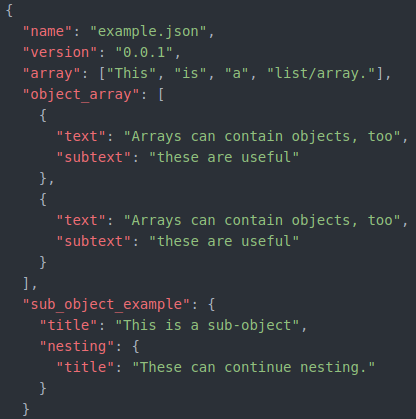
\includegraphics[width=4in]{images/Thesis_JSON.png}
    \caption{JSON excerpt from Beestream's package.json file.}
    \label{fig:json}
 \end{figure}
JSON or JavaScript Object Notation \cite{json} is a data interchange format that is heavily integrated with JavaScript.  The notation is intended to be human-readable, simple, and textual.  It is also used by JavaScript for most object representation.  It is simply constructed of objects that open with a single { (curly brace) followed by a series of comma-separated key-value pairs in the format key : value and closed by a single } (curly brace).  It can also contain lists defined by an opening [ (square bracket) followed by a list of comma separated values or objects and closed with a ] (square bracket).  Part of Beestream’s package.json can be seen in Figure \ref{fig:json} as an example of JSON. This means that JavaScript can be used for anything from data transmission or storage in a web application to human-defined configuration files for web servers and clients.  Due to its simplicity and deep integration into JavaScript, JSON is typically at the core of any JavaScript based application. \par

\subsection{Socket.io & WebSockets}
Socket.io \cite{socket} is a package distributed through NPM that utilizes the WebSocket protocol to offer bi-directional communication channels between a server and a client.  Socket.io provides valuable abstractions for the server and client to setup and communicate through WebSockets.  Socket.io is stable, performs well, and is widely used.  Beestream utilizes Socket.io for most server-client communications due to its simplicity and performance. \par

\subsection{Angular}
Angular \cite{angular} is a client-side application framework built in TypeScript.  TypeScript \cite{typescript} is a strongly typed superscript of JavaScript that compiles into plain JavaScript.  One of Angular’s primary features is its strict enforcement of the MVC architecture with modules, components, and a rendered view.  Angular seeks to provide the developer controlled access to the HTML document and a reliable and secure experience.  Because Angular controls the document, it can provide useful features such as a module-component structure, template-based rendering, and a router to render the appropriate components based on the current URL.  Angular also offers easy support for dynamic content with simple two-way data mapping from the client TypeScript to the rendered document.  Fundamentally, Angular tries to offer a reliable framework for building applications using TypeScript/JavaScript with certain stability and security guarantees.  Other frameworks, such as Vue and React, have seen wide use and can be interchanged with Angular in most applications.  Beestream uses Angular as it’s client-side framework. \par

\subsection{MongoDB}
MongoDB \cite{mongo} is a NoSQL database solution that utilizes BSON (Binary JSON) for data storage.  MongoDB provides a good read-write performance balance and allows for flexibility in the data types and formats that are stored.  Above all, MongoDB integrates well with JavaScript and returns JSON-formatted results that can be immediately accessed and used within a web server or client. \par
 \label{bkgrnd_technical}
				\section{Application Background}
				%
% bkgrnd_application.tex
%

	Our architecture was applied as part of the Beestream web application.  In order to understand the motivations for this project, the reader should have a general understanding of the Beemon project.  Beemon is a honey bee hive monitoring application that records video, audio, and temperature/humidity data at the entrance of a honeybee hive.  The recorded data is uploaded to a remote server where it can be accessed and analyzed.  As part of the Beemon project, a number of automated video and audio analytics programs were created.  These applications produce quantitative data, such as beehive arrivals and departures, from qualitative video and audio data.  When video or audio data is uploaded to the server, it is ingested into a MongoDB database and analyzed using these analytics programs.  The analysis results are included in the MongoDB database.  Beestream’s original purpose was to allow users to stream the video recorded by Beemon through a web application and comment/tag videos with interesting observations.  Given the readily available analysis, the idea was presented that Beestream could include various visualizations of the live honey bee hive data such as arrivals, departures, and temperature/humidity.  Our architecture was developed and applied to this visualization problem. \par
 \label{bkgrnd_application}

	\chapter[Methodology]{\centering Methodology} \label{methods}
	%
% methods_intro.tex
%

Methodology \label{methods_intro}
		\section{Equations}
		%
% methods_equations.tex
%

Some aligned, numbered equations:
\begin{align}
\mathbf{\hat{x}} &= \argmin_{\mathbf{x}}{\Vert \mathbf{Ax} - \mathbf{b} \Vert}\\
c^2 &= a^2 + b^2\\
f(x) &= \sum_{i=0}^{\infty}{\frac{f^{(i)}(0)}{i!}x^i}
\end{align} \label{methods_equations}

	\chapter[Results]{\centering Results} \label{results}
	%
% results_intro.tex
%

Our architecture sought to provide a generalized, adaptable, and extensible solution to the problem of web-based data visualization.  In order to demonstrate the practicality effectiveness of our architecture, we’ll overview the procedure to extend the Beestream web application.  The following sections will cover different common avenues of change for web-based data visualization applications and how our architecture accommodates these changes.  In most cases, the Beestream application will be discussed as an example. \par
 \label{results_intro}
		\section{Figures}
		% 
% results_figures.tex
% 

Some of your results may be figures, as seen in Figure \ref{fig:scatter}. (Discuss every figure in the text.)

\begin{figure}
    \centering
    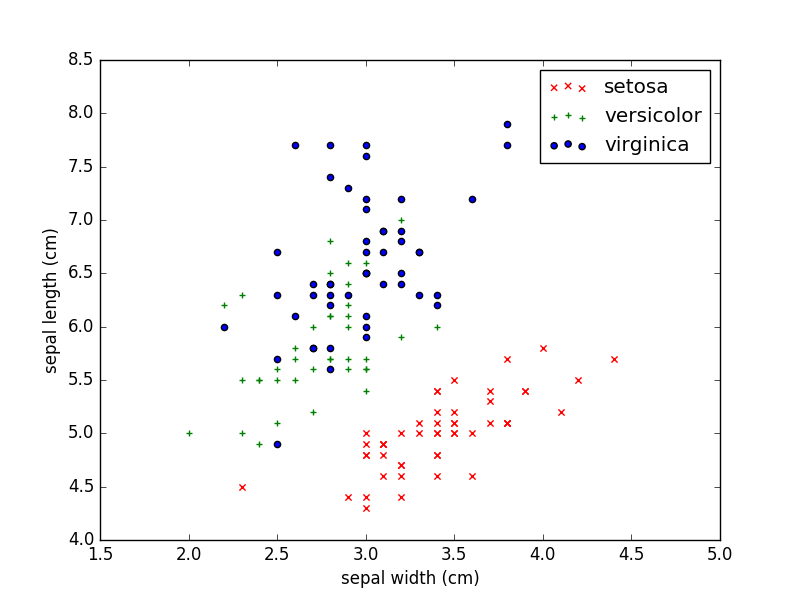
\includegraphics[width=4in]{images/scatter.png}
    \caption{This is a scatter plot.}
    \label{fig:scatter}
 \end{figure} \label{results_figures}
		\section{Tables}
		\begin{singlespace}
    \begin{longtable}{L{7cm}|L{7cm}}
    \caption{\textit{Country populations}}
    \label{tab:table}\\
      \textbf{COUNTRY} & \textbf{POPULATION}\\
      \hline
      \endhead
      China & 1,382,323,332\\
      \hline
      India & 1,326,801,576\\
      \hline
      United States & 324,118,787\\
      \hline
      Indonesia & 260,581,100\\
      \hline
    \end{longtable}
\end{singlespace} \label{results_tables}

	\chapter[Conclusion and Future Work]{\centering Conclusion and Future Work} \label{concl_futwork}
		\section{Conclusion}
		%
% concl.tex
%
Our proposed generalized architecture for web-based data visualizaiton meets all outlined objectives as is illustrated by the BeeStream web application.  Our architecture provides sufficient modularity for data sources and datasets, different data scales, data transmission, and charts while remaining general enough to be applicable across various client and server-side web frameworks.  BeeStream not only illustrates the capabilities and practicality of this architecture, but also serves as a basis for easy extension.  BeeStream, and the underlying architecture, met or exceeded our expectations for modularity and adaptability.  \par

Our future work revolves around utilizing our implemneted framework to build visualizations for more complex and varied data and generalizing our solution so that others can easily build applications using our architecture.  A potential extension for BeeStream would be a chart that allows the user to dynamically request datasets, which the driver would then request and serve as defined in our architecture.  Further future work would include building a ``boilerplate'' or starter application that contains the basic components of this architecture.  This starter application should be reproduced in each of the commonly used server and client-side web frameworks in order to accomodate as many developers as possible.  It would also be beneficial to build default \textit{ChartComponents} for each of the major charting library, as library interfaces vary.  Future research can be completed to produce starter code across as many platforms as possible so that others can easily build off of our work.
 \label{concl}
		\section{Future Work}
		%
% futwork.tex
%

Future work \label{futwork}

	\newpage

        \newlinestretch{1}
	\addcontentsline{toc}{chapter}{Bibliography}
        \bibliographystyle{plain}
	\bibliography{biblio}

	\appendix
	\fontsize{11pt}{26pt}\selectfont

	\chapter[Appendix]{\centering Appendix}
		%
% otherstuff.tex
%

You might use an appendix to dump in some source code.

\begin{singlespace}
\begin{verbatim} 
public class Hello
{
   public static void main(String[] args) {
      System.out.println("Hello world!");
   }
}
\end{verbatim} 
\end{singlespace} \label{otherstuff}


	\newpage
	\addcontentsline{toc}{chapter}{Vita}
		\chapter*{Vita}

Vita
\end{document}
